\item Let $\vec{O}$ be the centre and  $r$ be the radius.  For 
\begin{align}
\vec{A} = \myvec{2\\-2}, \vec{B} = \myvec{3\\4},
\end{align}

\begin{align}
\implies \norm{\vec{A}-\vec{O}} = \norm{\vec{B}-\vec{O}} &= r
\\
\implies \norm{\vec{A}-\vec{O}}^2 - \norm{\vec{B}-\vec{O}}^2  &= 0
\\
\implies \brak{\vec{A}-\vec{B}}^T\vec{O} &=   \frac{\norm{\vec{A}}^2- \norm{\vec{B}}^2}{2}
\\
\text{or, } \myvec{1 & 6}\vec{O} &= \frac{17}{2}
\label{eq:4.1.3points_circle1}
\end{align}
Also centre O lies on the line in \eqref{eq:4.1.3_line}
%
\begin{align}
\myvec{1&1} \vec{O} = 2
\label{eq:4.1.3line_circle1}
\end{align}
\eqref{eq:4.1.3points_circle1} and \eqref{eq:4.1.3line_circle1} result in the matrix equation
\begin{align}
\myvec{1 & 6 \\ 1 & 1}\vec{O} = \myvec{\frac{17}{2}\\2}
\label{eq:4.1.3finding_centre1}
\end{align}
%
The following code calculates centre and radius and plots figure \ref{fig:4.1.3_circle1}
\begin{lstlisting}
solutions/3/codes/circle1/circle1.py.py
\end{lstlisting}
\begin{figure}[!ht]
\centering
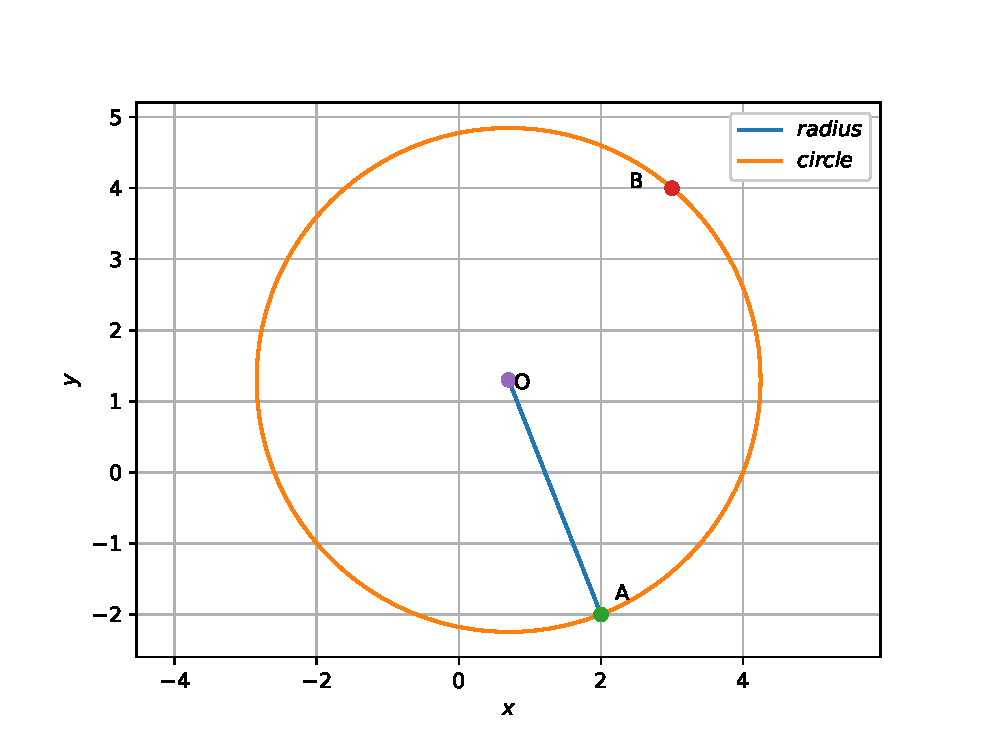
\includegraphics[width=\columnwidth]{./solutions/3/codes/circle1/pyfigs/circle1.eps}
\caption{Circle with centre at $\vec{O}$ and radius r}
\label{fig:4.1.3_circle1}
\end{figure}

